\documentclass{standalone}
\usepackage{tikz}
\usetikzlibrary{patterns, positioning}


\begin{document}
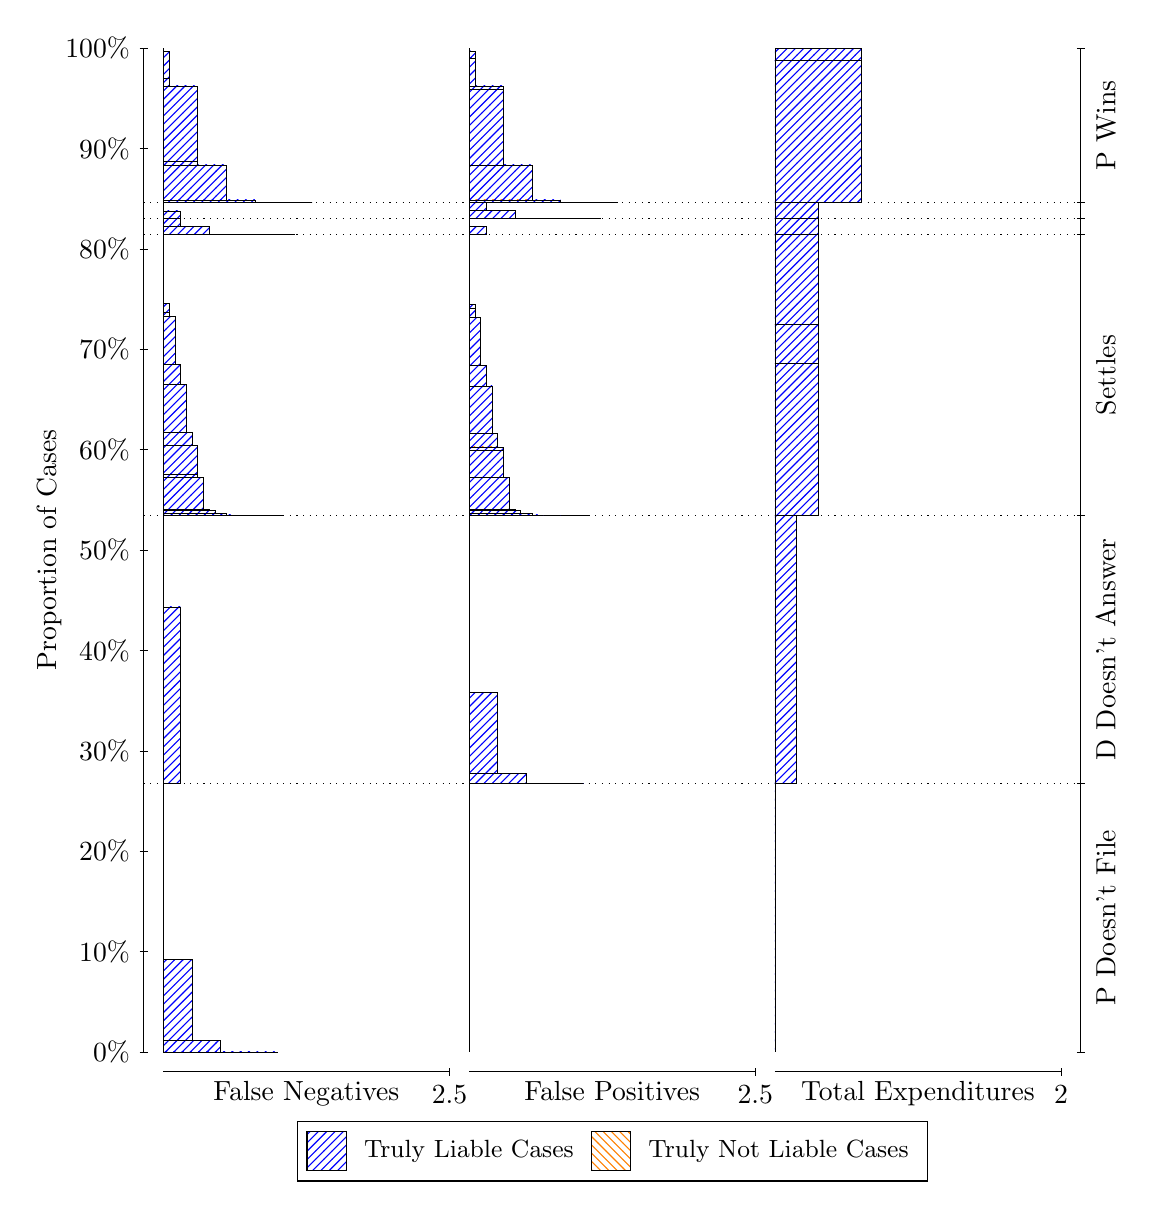
\begin{tikzpicture}
\draw[black, very thin] (1.5,1.75) -- (1.5,14.5);
\node[rotate=90, text=black, anchor=center] at (0.3, 8.125) {Proportion of Cases};
\draw[black, very thin] (1.45,1.75) -- (1.55,1.75);
\node[text=black, anchor=east] at (1.45, 1.75) {0\%};
\draw[black, very thin] (1.45,3.025) -- (1.55,3.025);
\node[text=black, anchor=east] at (1.45, 3.025) {10\%};
\draw[black, very thin] (1.45,4.3) -- (1.55,4.3);
\node[text=black, anchor=east] at (1.45, 4.3) {20\%};
\draw[black, very thin] (1.45,5.575) -- (1.55,5.575);
\node[text=black, anchor=east] at (1.45, 5.575) {30\%};
\draw[black, very thin] (1.45,6.85) -- (1.55,6.85);
\node[text=black, anchor=east] at (1.45, 6.85) {40\%};
\draw[black, very thin] (1.45,8.125) -- (1.55,8.125);
\node[text=black, anchor=east] at (1.45, 8.125) {50\%};
\draw[black, very thin] (1.45,9.4) -- (1.55,9.4);
\node[text=black, anchor=east] at (1.45, 9.4) {60\%};
\draw[black, very thin] (1.45,10.675) -- (1.55,10.675);
\node[text=black, anchor=east] at (1.45, 10.675) {70\%};
\draw[black, very thin] (1.45,11.95) -- (1.55,11.95);
\node[text=black, anchor=east] at (1.45, 11.95) {80\%};
\draw[black, very thin] (1.45,13.225) -- (1.55,13.225);
\node[text=black, anchor=east] at (1.45, 13.225) {90\%};
\draw[black, very thin] (1.45,14.5) -- (1.55,14.5);
\node[text=black, anchor=east] at (1.45, 14.5) {100\%};

\draw[black, very thin] (13.4,1.75) -- (13.4,14.5);
\draw[black, very thin] (13.35,1.75) -- (13.45,1.75);
\node[anchor=west] at (13.35, 1.75) {};
\draw[black, very thin] (13.35,5.1633) -- (13.45,5.1633);
\node[anchor=west] at (13.35, 5.1633) {};
\draw[black, very thin] (13.35,8.5605) -- (13.45,8.5605);
\node[anchor=west] at (13.35, 8.5605) {};
\draw[black, very thin] (13.35,12.134) -- (13.45,12.134);
\node[anchor=west] at (13.35, 12.134) {};
\draw[black, very thin] (13.35,12.336) -- (13.45,12.336);
\node[anchor=west] at (13.35, 12.336) {};
\draw[black, very thin] (13.35,12.537) -- (13.45,12.537);
\node[anchor=west] at (13.35, 12.537) {};
\draw[black, very thin] (13.35,14.5) -- (13.45,14.5);
\node[anchor=west] at (13.35, 14.5) {};

\draw[black, very thin, pattern color=blue, pattern=north east lines] (1.75,1.75) rectangle (3.2033,1.75);
\draw[black, very thin, pattern color=blue, pattern=north east lines] (1.75,1.75) rectangle (2.84,1.7512);
\draw[black, very thin, pattern color=blue, pattern=north east lines] (1.75,1.7512) rectangle (2.4767,1.8982);
\draw[black, very thin, pattern color=blue, pattern=north east lines] (1.75,1.8982) rectangle (2.1133,2.9236);
\draw[black, very thin, pattern color=orange, pattern=north west lines] (1.75,2.9236) rectangle (1.75,2.9236);
\draw[black, very thin, pattern color=blue, pattern=north east lines] (1.75,2.9236) rectangle (1.75,5.1633);
\draw[black, very thin, pattern color=blue, pattern=north east lines] (1.75,5.1633) rectangle (1.968,7.4037);
\draw[black, very thin, pattern color=orange, pattern=north west lines] (1.75,7.4037) rectangle (1.75,7.4037);
\draw[black, very thin, pattern color=blue, pattern=north east lines] (1.75,7.4037) rectangle (1.75,8.5605);
\draw[black, very thin, pattern color=blue, pattern=north east lines] (1.75,8.5605) rectangle (3.276,8.5605);
\draw[black, very thin, pattern color=blue, pattern=north east lines] (1.75,8.5605) rectangle (2.9853,8.5605);
\draw[black, very thin, pattern color=blue, pattern=north east lines] (1.75,8.5605) rectangle (2.9127,8.5605);
\draw[black, very thin, pattern color=blue, pattern=north east lines] (1.75,8.5605) rectangle (2.84,8.5605);
\draw[black, very thin, pattern color=blue, pattern=north east lines] (1.75,8.5605) rectangle (2.6947,8.5605);
\draw[black, very thin, pattern color=blue, pattern=north east lines] (1.75,8.5605) rectangle (2.622,8.572);
\draw[black, very thin, pattern color=blue, pattern=north east lines] (1.75,8.572) rectangle (2.5493,8.5931);
\draw[black, very thin, pattern color=blue, pattern=north east lines] (1.75,8.5931) rectangle (2.4767,8.5936);
\draw[black, very thin, pattern color=blue, pattern=north east lines] (1.75,8.5936) rectangle (2.404,8.6261);
\draw[black, very thin, pattern color=blue, pattern=north east lines] (1.75,8.6261) rectangle (2.3313,8.6457);
\draw[black, very thin, pattern color=blue, pattern=north east lines] (1.75,8.6457) rectangle (2.2587,9.0492);
\draw[black, very thin, pattern color=blue, pattern=north east lines] (1.75,9.0492) rectangle (2.186,9.0915);
\draw[black, very thin, pattern color=blue, pattern=north east lines] (1.75,9.0915) rectangle (2.186,9.449);
\draw[black, very thin, pattern color=blue, pattern=north east lines] (1.75,9.449) rectangle (2.1133,9.6153);
\draw[black, very thin, pattern color=blue, pattern=north east lines] (1.75,9.6153) rectangle (2.0407,10.227);
\draw[black, very thin, pattern color=blue, pattern=north east lines] (1.75,10.227) rectangle (1.968,10.487);
\draw[black, very thin, pattern color=blue, pattern=north east lines] (1.75,10.487) rectangle (1.8953,11.093);
\draw[black, very thin, pattern color=blue, pattern=north east lines] (1.75,11.093) rectangle (1.8227,11.146);
\draw[black, very thin, pattern color=blue, pattern=north east lines] (1.75,11.146) rectangle (1.8227,11.261);
\draw[black, very thin, pattern color=blue, pattern=north east lines] (1.75,11.261) rectangle (1.75,11.303);
\draw[black, very thin, pattern color=orange, pattern=north west lines] (1.75,11.303) rectangle (1.75,11.303);
\draw[black, very thin, pattern color=blue, pattern=north east lines] (1.75,11.303) rectangle (1.75,12.134);
\draw[black, very thin, pattern color=blue, pattern=north east lines] (1.75,12.134) rectangle (3.4213,12.134);
\draw[black, very thin, pattern color=blue, pattern=north east lines] (1.75,12.134) rectangle (3.058,12.134);
\draw[black, very thin, pattern color=blue, pattern=north east lines] (1.75,12.134) rectangle (2.6947,12.136);
\draw[black, very thin, pattern color=blue, pattern=north east lines] (1.75,12.136) rectangle (2.3313,12.238);
\draw[black, very thin, pattern color=blue, pattern=north east lines] (1.75,12.238) rectangle (1.968,12.336);
\draw[black, very thin, pattern color=orange, pattern=north west lines] (1.75,12.336) rectangle (1.75,12.336);
\draw[black, very thin, pattern color=blue, pattern=north east lines] (1.75,12.336) rectangle (1.968,12.433);
\draw[black, very thin, pattern color=orange, pattern=north west lines] (1.75,12.433) rectangle (1.75,12.433);
\draw[black, very thin, pattern color=blue, pattern=north east lines] (1.75,12.433) rectangle (1.75,12.537);
\draw[black, very thin, pattern color=blue, pattern=north east lines] (1.75,12.537) rectangle (3.6393,12.537);
\draw[black, very thin, pattern color=blue, pattern=north east lines] (1.75,12.537) rectangle (3.276,12.537);
\draw[black, very thin, pattern color=blue, pattern=north east lines] (1.75,12.537) rectangle (2.9127,12.571);
\draw[black, very thin, pattern color=blue, pattern=north east lines] (1.75,12.571) rectangle (2.5493,13.017);
\draw[black, very thin, pattern color=blue, pattern=north east lines] (1.75,13.017) rectangle (2.186,13.06);
\draw[black, very thin, pattern color=blue, pattern=north east lines] (1.75,13.06) rectangle (2.186,14.02);
\draw[black, very thin, pattern color=blue, pattern=north east lines] (1.75,14.02) rectangle (1.8227,14.111);
\draw[black, very thin, pattern color=blue, pattern=north east lines] (1.75,14.111) rectangle (1.8227,14.465);
\draw[black, very thin, pattern color=orange, pattern=north west lines] (1.75,14.465) rectangle (1.75,14.465);
\draw[black, very thin, pattern color=blue, pattern=north east lines] (1.75,14.465) rectangle (1.75,14.5);
\draw[black, very thin, pattern color=orange, pattern=north west lines] (5.6333,1.75) rectangle (5.6333,1.75);
\draw[black, very thin, pattern color=blue, pattern=north east lines] (5.6333,1.75) rectangle (5.6333,5.1633);
\draw[black, very thin, pattern color=orange, pattern=north west lines] (5.6333,5.1633) rectangle (7.0867,5.1633);
\draw[black, very thin, pattern color=blue, pattern=north east lines] (5.6333,5.1633) rectangle (7.0867,5.1633);
\draw[black, very thin, pattern color=blue, pattern=north east lines] (5.6333,5.1633) rectangle (6.7233,5.1636);
\draw[black, very thin, pattern color=blue, pattern=north east lines] (5.6333,5.1636) rectangle (6.36,5.2928);
\draw[black, very thin, pattern color=blue, pattern=north east lines] (5.6333,5.2928) rectangle (5.9967,6.3201);
\draw[black, very thin, pattern color=blue, pattern=north east lines] (5.6333,6.3201) rectangle (5.6333,8.5605);
\draw[black, very thin, pattern color=orange, pattern=north west lines] (5.6333,8.5605) rectangle (7.1593,8.5605);
\draw[black, very thin, pattern color=blue, pattern=north east lines] (5.6333,8.5605) rectangle (7.1593,8.5605);
\draw[black, very thin, pattern color=orange, pattern=north west lines] (5.6333,8.5605) rectangle (6.8687,8.5605);
\draw[black, very thin, pattern color=blue, pattern=north east lines] (5.6333,8.5605) rectangle (6.8687,8.5605);
\draw[black, very thin, pattern color=blue, pattern=north east lines] (5.6333,8.5605) rectangle (6.796,8.5605);
\draw[black, very thin, pattern color=orange, pattern=north west lines] (5.6333,8.5605) rectangle (6.7233,8.5605);
\draw[black, very thin, pattern color=blue, pattern=north east lines] (5.6333,8.5605) rectangle (6.7233,8.5605);
\draw[black, very thin, pattern color=orange, pattern=north west lines] (5.6333,8.5605) rectangle (6.578,8.5605);
\draw[black, very thin, pattern color=blue, pattern=north east lines] (5.6333,8.5605) rectangle (6.578,8.5605);
\draw[black, very thin, pattern color=blue, pattern=north east lines] (5.6333,8.5605) rectangle (6.5053,8.572);
\draw[black, very thin, pattern color=blue, pattern=north east lines] (5.6333,8.572) rectangle (6.4327,8.5923);
\draw[black, very thin, pattern color=orange, pattern=north west lines] (5.6333,8.5923) rectangle (6.4327,8.5923);
\draw[black, very thin, pattern color=blue, pattern=north east lines] (5.6333,8.5923) rectangle (6.4327,8.5924);
\draw[black, very thin, pattern color=blue, pattern=north east lines] (5.6333,8.5924) rectangle (6.36,8.5929);
\draw[black, very thin, pattern color=orange, pattern=north west lines] (5.6333,8.5929) rectangle (6.2873,8.5929);
\draw[black, very thin, pattern color=blue, pattern=north east lines] (5.6333,8.5929) rectangle (6.2873,8.6251);
\draw[black, very thin, pattern color=blue, pattern=north east lines] (5.6333,8.6251) rectangle (6.2147,8.6404);
\draw[black, very thin, pattern color=blue, pattern=north east lines] (5.6333,8.6404) rectangle (6.142,9.043);
\draw[black, very thin, pattern color=blue, pattern=north east lines] (5.6333,9.043) rectangle (6.0693,9.392);
\draw[black, very thin, pattern color=blue, pattern=north east lines] (5.6333,9.392) rectangle (6.0693,9.4341);
\draw[black, very thin, pattern color=orange, pattern=north west lines] (5.6333,9.4341) rectangle (5.9967,9.4341);
\draw[black, very thin, pattern color=blue, pattern=north east lines] (5.6333,9.4341) rectangle (5.9967,9.6018);
\draw[black, very thin, pattern color=blue, pattern=north east lines] (5.6333,9.6018) rectangle (5.924,10.208);
\draw[black, very thin, pattern color=blue, pattern=north east lines] (5.6333,10.208) rectangle (5.8513,10.468);
\draw[black, very thin, pattern color=blue, pattern=north east lines] (5.6333,10.468) rectangle (5.7787,11.08);
\draw[black, very thin, pattern color=blue, pattern=north east lines] (5.6333,11.08) rectangle (5.706,11.193);
\draw[black, very thin, pattern color=blue, pattern=north east lines] (5.6333,11.193) rectangle (5.706,11.246);
\draw[black, very thin, pattern color=blue, pattern=north east lines] (5.6333,11.246) rectangle (5.6333,12.134);
\draw[black, very thin, pattern color=orange, pattern=north west lines] (5.6333,12.134) rectangle (5.8513,12.134);
\draw[black, very thin, pattern color=blue, pattern=north east lines] (5.6333,12.134) rectangle (5.8513,12.232);
\draw[black, very thin, pattern color=blue, pattern=north east lines] (5.6333,12.232) rectangle (5.6333,12.336);
\draw[black, very thin, pattern color=orange, pattern=north west lines] (5.6333,12.336) rectangle (7.3047,12.336);
\draw[black, very thin, pattern color=blue, pattern=north east lines] (5.6333,12.336) rectangle (7.3047,12.336);
\draw[black, very thin, pattern color=blue, pattern=north east lines] (5.6333,12.336) rectangle (6.9413,12.336);
\draw[black, very thin, pattern color=blue, pattern=north east lines] (5.6333,12.336) rectangle (6.578,12.338);
\draw[black, very thin, pattern color=blue, pattern=north east lines] (5.6333,12.338) rectangle (6.2147,12.439);
\draw[black, very thin, pattern color=blue, pattern=north east lines] (5.6333,12.439) rectangle (5.8513,12.537);
\draw[black, very thin, pattern color=orange, pattern=north west lines] (5.6333,12.537) rectangle (7.5227,12.537);
\draw[black, very thin, pattern color=blue, pattern=north east lines] (5.6333,12.537) rectangle (7.5227,12.537);
\draw[black, very thin, pattern color=orange, pattern=north west lines] (5.6333,12.537) rectangle (7.1593,12.537);
\draw[black, very thin, pattern color=blue, pattern=north east lines] (5.6333,12.537) rectangle (7.1593,12.537);
\draw[black, very thin, pattern color=orange, pattern=north west lines] (5.6333,12.537) rectangle (6.796,12.537);
\draw[black, very thin, pattern color=blue, pattern=north east lines] (5.6333,12.537) rectangle (6.796,12.571);
\draw[black, very thin, pattern color=orange, pattern=north west lines] (5.6333,12.571) rectangle (6.4327,12.571);
\draw[black, very thin, pattern color=blue, pattern=north east lines] (5.6333,12.571) rectangle (6.4327,13.017);
\draw[black, very thin, pattern color=blue, pattern=north east lines] (5.6333,13.017) rectangle (6.0693,13.976);
\draw[black, very thin, pattern color=orange, pattern=north west lines] (5.6333,13.976) rectangle (6.0693,13.976);
\draw[black, very thin, pattern color=blue, pattern=north east lines] (5.6333,13.976) rectangle (6.0693,14.02);
\draw[black, very thin, pattern color=blue, pattern=north east lines] (5.6333,14.02) rectangle (5.706,14.374);
\draw[black, very thin, pattern color=blue, pattern=north east lines] (5.6333,14.374) rectangle (5.706,14.465);
\draw[black, very thin, pattern color=blue, pattern=north east lines] (5.6333,14.465) rectangle (5.6333,14.5);
\draw[black, very thin, pattern color=orange, pattern=north west lines] (9.5167,1.75) rectangle (9.5167,1.75);
\draw[black, very thin, pattern color=blue, pattern=north east lines] (9.5167,1.75) rectangle (9.5167,5.1633);
\draw[black, very thin, pattern color=orange, pattern=north west lines] (9.5167,5.1633) rectangle (9.7892,5.1633);
\draw[black, very thin, pattern color=blue, pattern=north east lines] (9.5167,5.1633) rectangle (9.7892,8.5605);
\draw[black, very thin, pattern color=orange, pattern=north west lines] (9.5167,8.5605) rectangle (10.062,8.5605);
\draw[black, very thin, pattern color=blue, pattern=north east lines] (9.5167,8.5605) rectangle (10.062,10.493);
\draw[black, very thin, pattern color=orange, pattern=north west lines] (9.5167,10.493) rectangle (10.062,10.493);
\draw[black, very thin, pattern color=blue, pattern=north east lines] (9.5167,10.493) rectangle (10.062,10.986);
\draw[black, very thin, pattern color=orange, pattern=north west lines] (9.5167,10.986) rectangle (10.062,10.986);
\draw[black, very thin, pattern color=blue, pattern=north east lines] (9.5167,10.986) rectangle (10.062,12.134);
\draw[black, very thin, pattern color=orange, pattern=north west lines] (9.5167,12.134) rectangle (10.062,12.134);
\draw[black, very thin, pattern color=blue, pattern=north east lines] (9.5167,12.134) rectangle (10.062,12.336);
\draw[black, very thin, pattern color=orange, pattern=north west lines] (9.5167,12.336) rectangle (10.062,12.336);
\draw[black, very thin, pattern color=blue, pattern=north east lines] (9.5167,12.336) rectangle (10.062,12.537);
\draw[black, very thin, pattern color=orange, pattern=north west lines] (9.5167,12.537) rectangle (10.607,12.537);
\draw[black, very thin, pattern color=blue, pattern=north east lines] (9.5167,12.537) rectangle (10.607,14.341);
\draw[black, very thin, pattern color=orange, pattern=north west lines] (9.5167,14.341) rectangle (10.607,14.341);
\draw[black, very thin, pattern color=blue, pattern=north east lines] (9.5167,14.341) rectangle (10.607,14.5);
\draw[black, dotted] (1.5,5.1633) -- (13.4,5.1633);
\draw[black, dotted] (1.5,8.5605) -- (13.4,8.5605);
\draw[black, dotted] (1.5,12.134) -- (13.4,12.134);
\draw[black, dotted] (1.5,12.336) -- (13.4,12.336);
\draw[black, dotted] (1.5,12.537) -- (13.4,12.537);
\draw[black, very thin] (1.75,1.5) -- (5.3833,1.5);
\node[text=black, anchor=north] at (3.5667, 1.5) {False Negatives};
\draw[black, very thin] (5.3833,1.45) -- (5.3833,1.55);
\node[text=black, anchor=north] at (5.3833, 1.45) {2.5};

\draw[black, very thin] (5.6333,1.5) -- (9.2667,1.5);
\node[text=black, anchor=north] at (7.45, 1.5) {False Positives};
\draw[black, very thin] (9.2667,1.45) -- (9.2667,1.55);
\node[text=black, anchor=north] at (9.2667, 1.45) {2.5};

\draw[black, very thin] (9.5167,1.5) -- (13.15,1.5);
\node[text=black, anchor=north] at (11.333, 1.5) {Total Expenditures};
\draw[black, very thin] (13.15,1.45) -- (13.15,1.55);
\node[text=black, anchor=north] at (13.15, 1.45) {2};

\node[text=black, centered, rotate=90] at (13.72, 3.4566) {P Doesn't File};
\node[text=black, centered, rotate=90] at (13.72, 6.8619) {D Doesn't Answer};
\node[text=black, centered, rotate=90] at (13.72, 10.347) {Settles};


\node[text=black, centered, rotate=90] at (13.72, 13.518) {P Wins};

\draw (7.449999999999999,1.5) node[draw=none] (baseCoordinate) {};
\begin{scope}[align=center]
        \matrix[scale=0.5, draw=black, below=0.5cm of baseCoordinate, nodes={draw}, column sep=0.1cm]{
            \node[rectangle, draw, minimum width=0.5cm, minimum height=0.5cm, pattern color=blue, pattern=north east lines] {}; &
            \node[draw=none, font=\small, text=black] (B) {Truly Liable Cases}; &
            \node[rectangle, draw, minimum width=0.5cm, minimum height=0.5cm, pattern color=orange, pattern=north west lines] {}; &
            \node[draw=none, font=\small, text=black] (B) {Truly Not Liable Cases}; \\
            };
\end{scope}

\end{tikzpicture}
\end{document}